\listfiles
\documentclass[twoside,12pt]{article}
\newcommand{\dataset}{{\cal D}}
\newcommand{\fracpartial}[2]{\frac{\partial #1}{\partial  #2}}
\usepackage{hyperref}
\usepackage{enumerate}
\usepackage[top=2in, bottom=1.5in, left=0.85in, right=0.5in]{geometry}
\usepackage[hyphenbreaks]{breakurl}
%\usepackage[pdfstartview=FitH,pdfstartpage=13,pdfpagemode=UseNone]{hyperref}
\usepackage{amsfonts}
\usepackage{graphicx} 
\usepackage[linesnumbered,ruled]{algorithm2e}
\usepackage{float}
\usepackage{amssymb,amsmath}
\usepackage{mdwlist }
\usepackage{color}
\usepackage{multirow}
\usepackage{listings}
\usepackage{float}
\usepackage{setspace}
\usepackage[english]{babel}

\usepackage{graphicx}
\usepackage{caption}
\usepackage{subcaption}


\definecolor{darkblue}{rgb}{0.0,0.0,0.5}
\newtheorem{Dfn}{Definition}
\hypersetup{colorlinks,breaklinks,
            linkcolor=darkblue,urlcolor=darkblue,
            anchorcolor=darkblue,citecolor=darkblue}
\newcommand{\sign}{\text{sign}}
\newcommand{\argmin}{\arg\!\max}
\begin{document}

\title{Latent Dirichlet Allocation for Document Topic Discovery\\  Learning Algorithms, Project 3}
\author{Mohsen Malmir, Erfan Sayyari}
\maketitle

\section{Abstract}
In this paper, a popular generative model called Latent Dirichlet Allocation (LDA) is used to discover the underlying topics of  a set of documents. Learning topics in documents is an unsupervised learning problem which exploits the frequency of words in documents. Gibbs sampling is used with Harmonic mean as a measure of goodness-of-fit to train the LDA model. We show the results of training the model using classic400 and DailyKOS blog datasets. In both cases, top words in the discovered topics and the distribution of topics in each document are represented. We also show that our model can predict the true label for topics for documents of classic400 dataset with more that 97\% accuracy.

\section{Introduction}
\par{Discovering the topics of documents is a well known problem in machine learning. The goal is to represent a document as a distribution over a set of topics. Usually the data comes in form of a huge corpus extracted from blogs or news websites. Because of that, the data comes without any accompanying training labels, meaning there are no sample topic or word distributions. For this unsupervised learning problem, Latent Dirichlet Allocation (LDA) model is proposed that learns the topics within a document along with the distribution of words in each document.}
\par{For LDA model, the likelihood of data given model can't be expressed in closed form. Because of this, we use Gibbs sampling as a technique to infer the parameters of the model. Gibbs sampling can be very time consuming, specifically because the number of random variables in the model is huge. To make the sampling faster, we use a version of the algorithm called collapsed Gibbs sampling. In this method, some of the random variables in the model are marginalized and sampling is thus required only for a subset of random variables in the model .}
\par{We train the proposed model with two different datasets, classic400 and DailyKOS blog. Classic400 dataset is small, and is accompanied by true labels for topics in documents. This is a suitable dataset to perform accuracy test on the model. We show that the proposed model with Gibbs sampling learns to predict the topic for each document with more than 97\% accuracy. For both datasets, we look into top words for each learned topic to see if they are logically related. As we see later in this report, the model can discover meaningful topics from unlabeled text corpus.}

\section{Design and Analysis of Algorithm}

\subsection{The bag-of-words representation for Documents}
A document is a collection of words and the structure that puts these words together. If we only look at words, we find some words that are not correlated with any topic. These are words that can be found in any document with any topic. Examples of these words are pronouns (you, he, it) connectives (and, because, however), prepositions (to, of, before), auxiliaries (have, been, can), and generic nouns (amount, part, nothing). For the purpose of topic selection, we discard these words from documents as clearly they don't help in picking the right topic. Then we take the union of all words in corpus and call it \emph{dictionary}.

In order to determine a topic for a document, we have to represent  documents using a set of features. We adapt a representation called \emph{bag of words}, in which each document is represented as a histogram over the dictionary. Let $V$ be the total number of words in the dictionary, then each document is represented as a $V$-dimensional vector $x$, where $x[i]$ is the number of times the $i$th word appeared in the document. We can calculate the length of the document as $n=\sum_{m}x_j.$

\subsection{Latent Dirichlet Allocation Model}
To learn the topic distribution for documents, we use the model shown in figure \ref{figGM}. This is a model of $M$ documents, each with length $n_m$. Each word in a document comes from a \emph{topic} $z$. A topic is modeled as a multinomial distribution over the dictionary, with $\phi_k$ as vector. Note that $\phi_k[i]$ denotes the probability that topic $k$ gives to the $i$th word in the dictionary. A document is modeled as a multinomial distribution over topics, with $\theta$ representing the parameters. Again, $\theta_m[i]$ represents the probability of having topic $i$ in the $m$th document. Finally, we put Dirichlet priors over document and topic distributions. The prior over documents is represented by the node $\alpha$, and denotes the prior belief in the distribution of topics in different documents. Also, the prior over topics is represented by node $\beta$, and denotes the prior belief of distribution of words in topics.

\begin{figure}[h!]
\centering
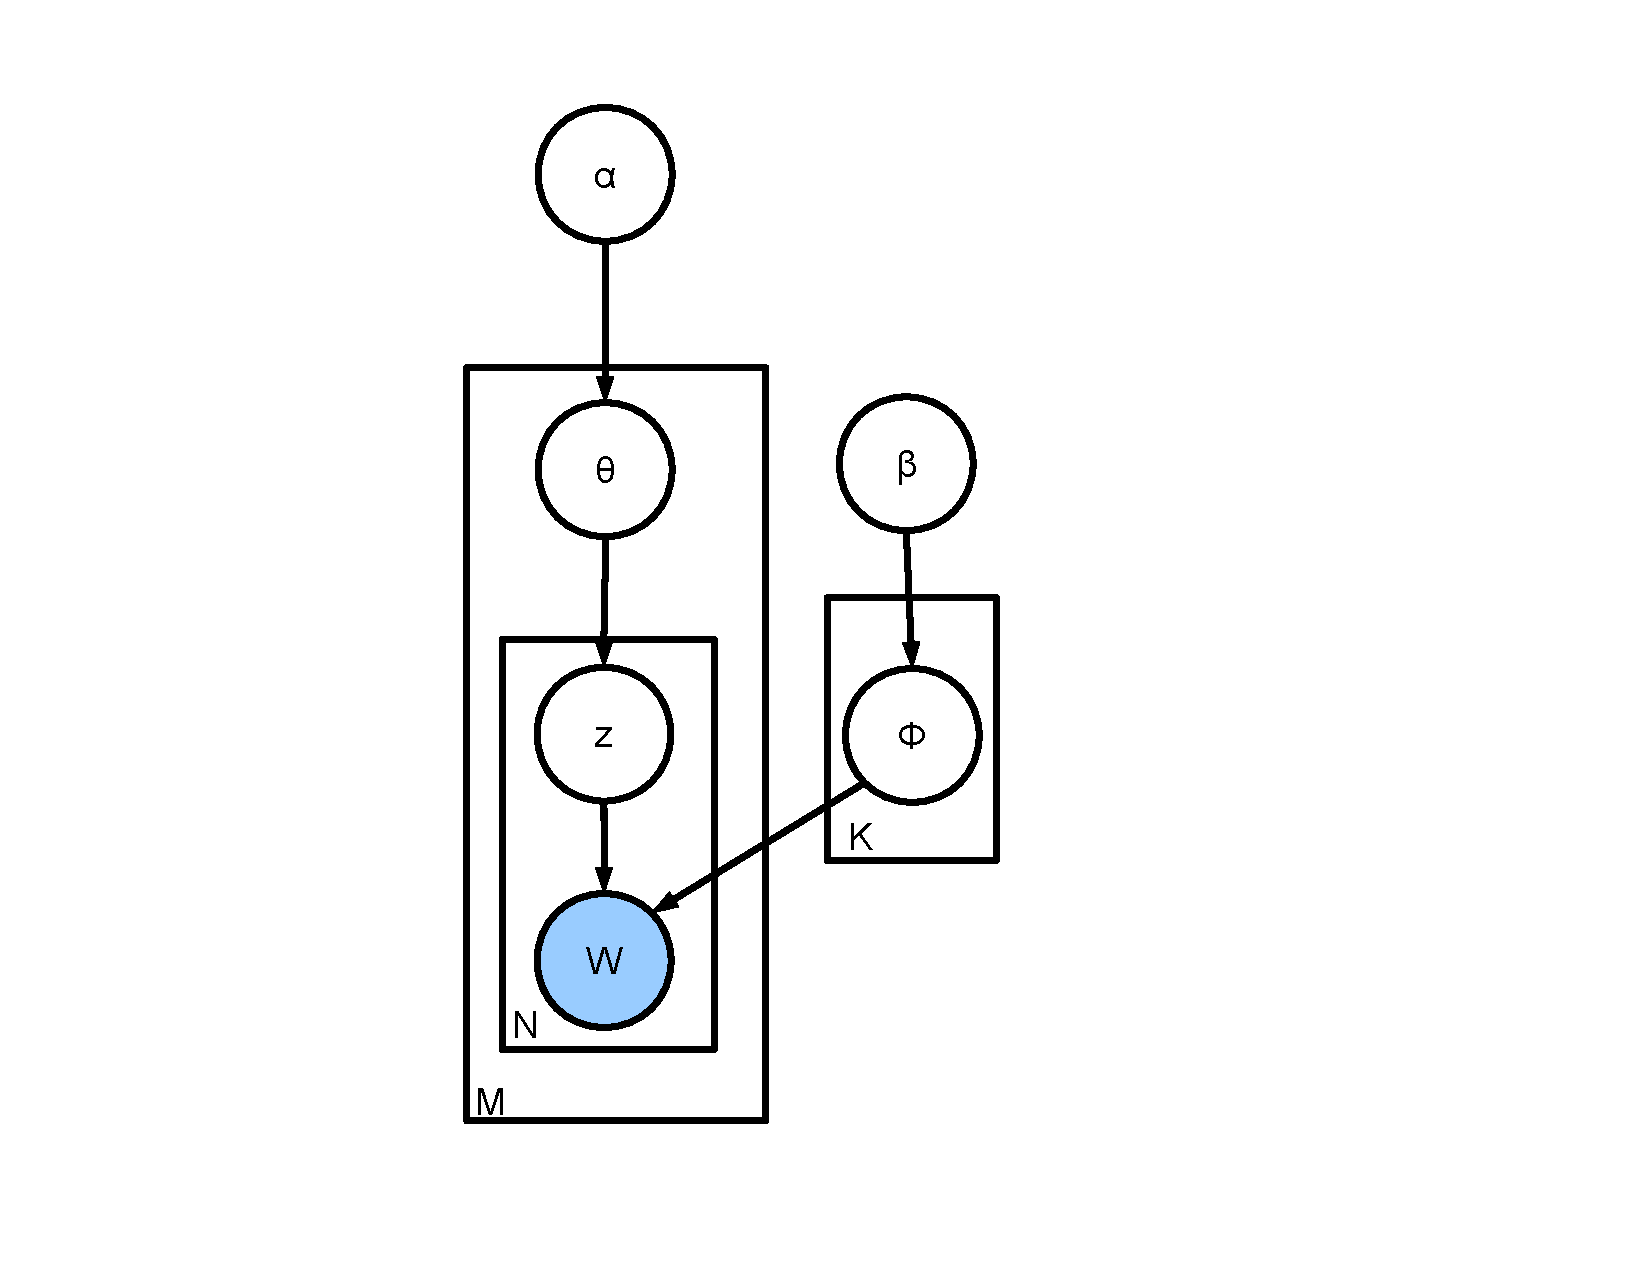
\includegraphics[width=.3\textwidth]{./figs/gm.pdf}
\caption{Plate notation of the LDA graphical model. The shaded node $w$ is observed. }
\label{figGM}
\end{figure}

The probability distribution represented by the graphical model in figure \ref{figGM} is,

\begin{align}
P(\alpha,\Theta,&Z,\beta,\Phi,W)  \\  &=P(\alpha) P(\beta) P(\Theta | \alpha) P(\Phi|\beta) P(Z|\Theta) P(W|Z,\Phi) \\ &= Dir(\alpha) Dir(\beta) \prod_{m=1}^M \text{Multi}(\theta_m | \alpha) \prod_{k=1}^K \text{Multi}(\phi_k | \beta) \prod_{t=1}^T \text{Multi}(w_t | \phi_{z_t})
\end{align}
 
 In the formula above, $\Phi = \{\phi_k, k=1,\ldots,K\}$ and $\Theta=\{\theta_m, m=1,\ldots,M\}$, $Dir$ represents Dirichlet and Multi represents the multinomial distributions. Also, $W = \{w_t, t=1,\ldots,T\}$ represents the entire set of words in the corpus. Note that the prior over topics and documents is chosen to be conjugate,
 
\begin{align}
\gamma \sim Dir(\alpha) \Rightarrow P(\gamma | \alpha) = \frac{\Gamma(\sum_{i=1}^M \alpha_i)}{\prod_{i=1}^M \Gamma(\alpha_i)} \prod_{i=1}^M \gamma_i^{\alpha_i -1} 
\end{align}
where
\begin{align}
\Gamma(t) = \int_0^\infty x^{t-1} e^{-x} dx
\end{align}
is the extension of Factorial function to continuous variables.
\subsection{ LDA Generative process}
To better understand the LDA model, we can look at how documents are generated in this model. First, $\phi_k, k=1,\ldots,K$ are randomly drawn from $Dir(\beta)$. Then For document $m, m=1,\ldots,M$, $\theta_m$ is sampled from $Dir(\alpha)$. Then $n_m$ topics are randomly drawn from Multi$(\theta_m)$. Given $z_t$, the $t$th word is selected from $\phi_{z_t}$. Remember that Gibbs sampling works by sampling from the posterior of variables, one variable at a time. 


Inference includes determining $\theta_m, \phi_k$ for $m=1,\ldots,M,\;\; k=1,\ldots,K$. Note that this is an unsupervised learning problem, where the training vectors are not accompanied by a target value. We propose a model, shown in figure \ref{figGM}, and we want to adapt the model parameters to the training data. A major drawback of the LDA topic model is that we cannot calculate the likelihood of the data analytically. In such situations, MCMC methods come to our help. Particularly, we use Gibbs sampling to infer the model parameters $\theta_m$ and $\phi_k$. First, note that we can integrate out $\theta$ and $\phi$ nodes of the LDA model. This is due to the fact that the distribution of $\alpha$ and $\theta$ are conjugate. Also, this is the case for $\beta$ and $\phi$. Since $w$ is observed, Gibbs sampling reduces to sampling $z_t$ nodes in the model. Given the current values for all other $z$ variables, which we call $Z_{-t}$, and all words $W$, we have
\begin{align}
p(z_t|Z_{-t},W)=\frac{p(Z,W)}{P(Z_{-t},W)}=\frac{p(W|Z)p(Z)}{p(w_t|Z_{-t})p(W_{-t}|Z_{-t})p(Z_{-t})}
\end{align}
In the lectures, it was shown that,
\begin{equation}
\label{eqZLikelihood}
p(z_t=j|Z_{-t},W)\propto \frac{q'_{jw_t}+\beta_{w_t}}{\sum_{t'} q'_{jw_{t'}}+\beta_{t'}}\frac{n'_{mj}+\alpha_j}{\sum_k n'_{mk}+\alpha_k}.
\end{equation}
where $m$ is the document to which $w_t$ belongs, $q'_{jw_{x}}$ is the number of times word $w_x$ appeared in topic $j$ and $n'_{mj}$ is the number of times topic $j$ was used in document $m$. Also $\alpha_x$ and $\beta_x$ refer the the $x$th element of vectors $\alpha$ and $\beta$ respectively.

After training is complete, we can calculate the probability of word $w$ under topic $k$ by,
\begin{equation}
\phi_{k,w}=\frac{q_{k,w}+\beta_{w}}{\sum_{w'} q_{kw'}+\beta_{w'}}
\end{equation}
 and the probability of topic $k$ in document $m$ using the following equation:
\begin{equation}
\theta_{m,k}=\frac{n_{mk}+\alpha_k}{\sum_{k'=1}^K n_{mk'}+\alpha_{k'}}.
\end{equation}


In each epoch we update the topic for all words by sampling from (\ref{eqZLikelihood}). In later sections in the details of implementation, we see that we can calculate (\ref{eqZLikelihood}) in constant time for each $z_t$. Therefor, time complexity of each epoch for Gibbs sampling is $O(NK)$, where $N$ is the total number of words in corpus and $K$ is the number of topics.


\subsection{Details of implementation}
\begin{algorithm}[h!]
\# initialization\;
 zero all count variables, $n_{m,k}$, $n_m$, $q_k^{(t)}$, $q_k$ \\
\For{all documents  $m\in{[1,M]}$}{
\For{all words $n \in{[1,N_m]}$ in document $m$}{
 	sample topic index $z_{m,n}=k\sim{Mult(\frac{1}{K})}$\\
	 increment document-topic count: $n_m^{(k)+1}$\\
	 increment document-topic sum: $n_m+1$\\
	 increment topic-term count: $q_k^{(t)}+1$\\
 	increment topic-term sum: $q_k+1$\\
}
}
\#Gibbs sampling\;
\While{not converged}{
	\For{all documents  $m\in{[1,M]}$}{
		\For{all words $n \in{[1,N_m]}$ in document $m$}{
\#for the current assignment of $k$ to a term $t$ for word $w_{m,n}$:\\
decrement counts and sums: $n_m^{(k)}-1,n_m-1,q_k^{(t)}-1,q_k-1$\\
\#multinomial sampling acc. to Equation 7:\\
sample topic index $\overline{k}\sim{p(z_i|,Z_{-i},W)}$\\
\#use the new assignment of $z_{m,n}$ to the term $t$ for word $w_{m,n}$ to:\\
increment counts and sums: $n_m^{(k)}+1,n_m+1,q_k^{(t)}+1,q_k+1$\\
	}
		}
\#check convergence and return multinomial parameters;\ \\
	\If{converged and $L$ iterations}{
return parameter set $\Phi$ according to Equation 8\\
return parameter set $\Theta$ according to Equation 9\\
	}
}

\caption{Gibbs sampling algorithm for latent Dirichlet allocation}
\label{algorithm}
\end{algorithm}

Algorithm~\ref{algorithm} describes a pseudocode that represents our implementation. Firstly, we initialize 4 different vectors that count number of each topic $k$ in document $m$ ($n_m^{(k)}$ with size $K\times M$. $K$ is the number of topics and $M$ is the number of documents.), total number of topics in document number $m$ ($n_m$ with length M, total number of documents), number of topics associated with term $t$ ($q_k^{(t)}$ with size $K\times V$, where $K$ is the total number of topics and $V$ is dictionary size), and the total occurrence of topic $k$ in the whole corpus ($q_k$ with length $K$, number of topics). Afterwards, we associate randomly selected topic indexes for each word in corpus according to $Mult(\frac{1}{K})$, where $Mult$ shows multinomial distribution. 

After initialization, we start Gibbs sampling. In order to assure convergence we set the number of iterations to be large enough. We consider different number of iterations, and for dataset Classic400 in order to give the best accuracy based on the maximum probable topic of each document, number of iterations equal to 500 is the best. 

In each epoch, we consider one document (say $m$) and word $n$ in this topic. We discard it from the corpus, and decrement the associated counts. Then we sample a topic from the multinomial distribution according to the the posterior probability of $p(z_i|Z_{-i},W)$, where $Z_{-i}$ indicates that the whole set of topic labels except topic label number $i$, and $W$ indicates the total set of words. Then we use the new assignment of $z_{m,n}$ to term $t$ for word $w_{m,n}$ to update associated counts ( $n_m^{(k)}+1,n_m+1,q_k^{(t)}+1,q_k+1$). 

After convergence according to large number of iteration, we return the parameter sets $\Phi$ and $\Theta$ according to Equation 8 and Equation 9.


\section{Design of Experiments}

\subsection{Dataset Selection}
The experiments on the model described above was done using two datasets: classic400 and dailyKOS. Table \ref{tableDatasetStats} display the number of documents, words and total number of words in these datasets. Classic400 is a small dataset, and the fact that it is accompanied by true labels makes it appealing for experiments. DailyKOS on the other hand is a larger dataset, and though it doesn't have the true labels, its large number of documents and total number of words makes it a good test to the performance of the proposed model. 


\begin{table}
\vspace{-2cm}
\center
\begin{tabular}{|c|c|c|}
\hline
 & \textbf{Classic400} & \textbf{DailyKOS} \\
 \hline
\textbf{ number of Documents} & 400 & 3430 \\
\textbf{ Dictionary Size} & 6205 & 6906 \\
\textbf{ Total Number of Words} & 31516 & 467714\\
 \hline
\end{tabular}
\caption{Statistics of classic400 and DailyKOS datasets.}
\label{tableDatasetStats}
\end{table}

\subsection{Harmonic Mean  as a Measures for Goodness-of-Fit}
Harmonic mean is proposed as a measure for goodness-of-fit for unsupervised models \cite{harmonic}. Harmonic mean is defined as:
\begin{equation}
\frac{1}{M}\sum_{m=1}^{M}(\frac{1}{K}\sum_{k=1}^{K}\theta_{m,k})^{-1}
\end{equation}
where $\theta_{m,k}$ is the topic distribution for document m and topic k. If the document distribution has higher probability for only some topics, its associated harmonic mean value would be lower. So, the model could have better ability to separate documents into different topics. In our experiments, we find that Harmonic mean is not a good measure for convergence, since its value converges after the very first few epochs. This is one of the difficulties with Harmonic mean, as it overestimates the goodness of model. This also has been noted before \cite{wallach}.


\subsection{Hyperparameters Selection}
There are two sets of hyper parameters in our model: $\alpha$ which is the parameters of the Dircihlet prior over documents and $\beta$ which is the vector of parameters for Dirichlet prior over topics. One way to select these parameters is to use expert knowledge in determining these parameters. In this case, the expert can give an estimate of the distribution of topics inside documents or distribution of words for different topics. Despite enriching the model, this method seems infeasible for us since we have no source of expertise in this area. Another way is to use an uninformative uniform prior, which acts as psuedo-counts to prevent technical difficulties.\\
Here, we adapt the same parameter values as \cite{fastlda}: $\alpha \in \{0.01,0.1\}$ and $\beta\in\{2/k,0.2/k\}$. These value make sense since they prefer sparse distributions for $\theta$ and $\phi$. Usually documents contain a few topics, therefore a document is usually a sparse distribution over topics. Also when the dictionary size is large, it makes sense to have a topic that is sparse, i.e. it gives higher probability to a few words. Besides the sparsity, there is no other information we are incorporating in our priors. 

\section{Results}


\subsection{Classic400}
We train 4 models on classic400 dataset using prior values mentioned before. Table \ref{tableClssicRecognition} shows the recognition rate for predicting the correct topic for documents in this dataset. For each document, we pick the topic with maximum probability as predicted topic for that document. Then all mappings from the predicted topics to the real topics are investigated. The results shown in table \ref{tableClassicRecognition} represent the best results found on this mapping. These rates indicate that the proposed model fits the data very well.

One should also note the effect of hyper parameters on recognition rates. Among four different values, the model with the lowest recognition rate is the for which the prior parameters enforce the least amount of sparsity of documents and topics. In our experiments, we tried less sparse values, eg. $\beta=10$, but the recognition rates were not good and the resulting topic distributions were a mix of different topics with no observable preference for a specific topic.

Measuring the goodness-of-fit for unsupervised models is a difficult task, however the structure of problem at hand can be exploited to investigate if the model has learned any meaningful pattern in the input data. For the present problem, we can observe if the set of words inside learned topics are semantically similar. Table \ref{tableTopWordsClassic} displays the top 20 words for each topic. It is interesting to look at this table, as the words in each row totally make sense. For example, the words in the third row represent the medical topic for documents.

Figure \ref{figClassicDist} shows the distribution of documents based on $\theta_m$. In this figure, document $m$ is represented in 3D space with the normalized count vector $\theta_m$ obtained from Gibbs sampling. The best recognition rate is obtained from the model shown in left side of bottom row in figure \ref{figClassicDist}. One thing to note here is that this is the most sparse representation of documents among all 4 models. For all figures here, the documents are mainly concentrated at vertices of the 2D simplex. 


\begin{table}[!]
\begin{center}
\begin{tabular}{| c | c |} 
\hline
\textbf{Hyper paramteres}& \textbf{Topic prediction rate}  \\ \hline

$\alpha=0.01,\beta=2.0$ & $0.9725$ \\ \hline
$\alpha=0.1,\beta=2.0$ &  $0.9375$ \\ \hline
$\alpha=0.01,\beta=0.2$ & $0.97$ \\ \hline
$\alpha=0.1,\beta=0.2$ & $0.96$ \\ \hline
 
\end{tabular}
\caption{Recognition rate for predicting the correct topic for each document for classic400 dataset.}
\label{tableClssicRecognition}
\end{center}
\end{table}

\begin{table}[h!]
\begin{center}
\begin{tabular}{| c | p{12cm} |}
\hline
\textbf{Topic}& \textbf{Top 20 Words}  \\ \hline
\textbf{1}&system, scientific, retrieval, research, language, science, journals,  methods, systems, subject, problems, requests, library, classification, data,  organization, general, development, publications, considered\\ \hline
\textbf{2}&boundary, layer, wing, mach, supersonic, wings, velocity, ratio, shock, effects, surface, plate, lift, jet, numbers, solution, edge, high, speeds, heat\\
 \hline
\textbf{3}&patients, ventricular, fatty, left, nickel, acids, cases, aortic, blood, glucose, normal, septal, visual, acid, pulmonary, defect, time, clinical, ffa, regurgitation\\
 \hline
 
\end{tabular}
\caption{Top 20 words for 3 topics of Classic400. Topic 1 is scientific methods, topic 2 is aerospace-physics and topic 3 is medical.}
\label{tableTopWordsClassic}
\end{center}
\end{table}




\begin{figure}[h!]
        \centering
        \begin{subfigure}[b]{0.5\textwidth}
                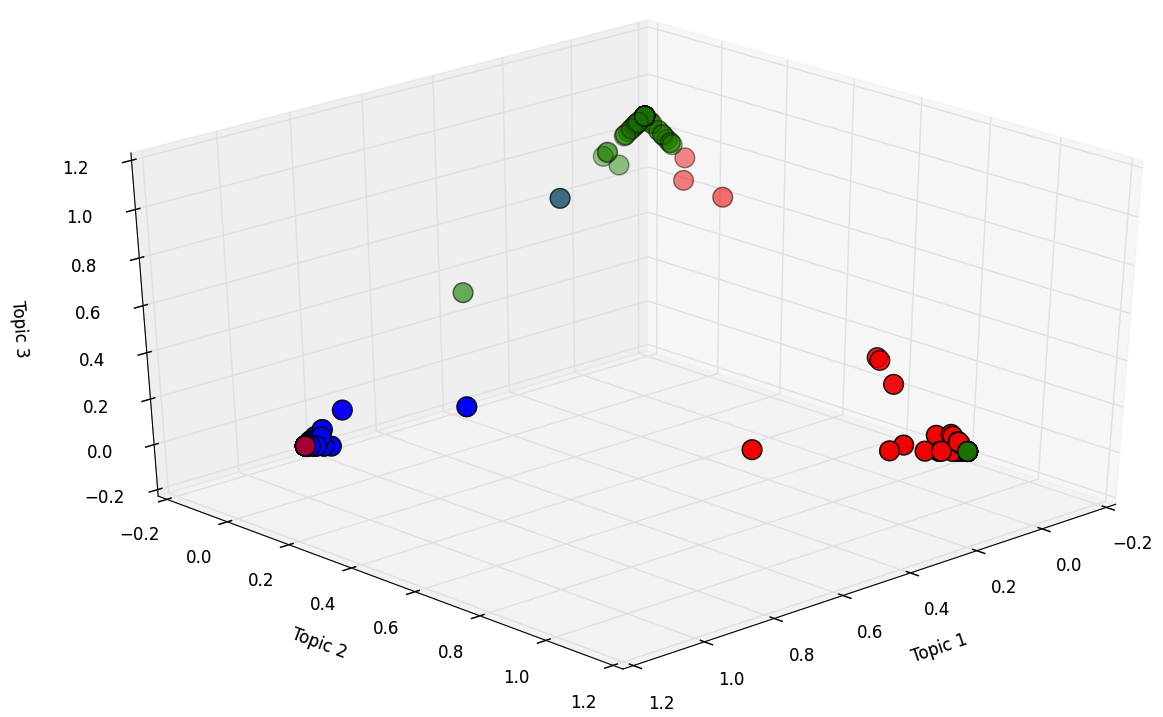
\includegraphics[width=\textwidth]{figs/classicalpha01beta2.png}
                \caption{$\alpha=0.1,\;\beta=2.$}
                \label{fig:gull}
        \end{subfigure}%
        ~ %add desired spacing between images, e. g. ~, \quad, \qquad etc.
          %(or a blank line to force the subfigure onto a new line)
        \begin{subfigure}[b]{0.5\textwidth}
                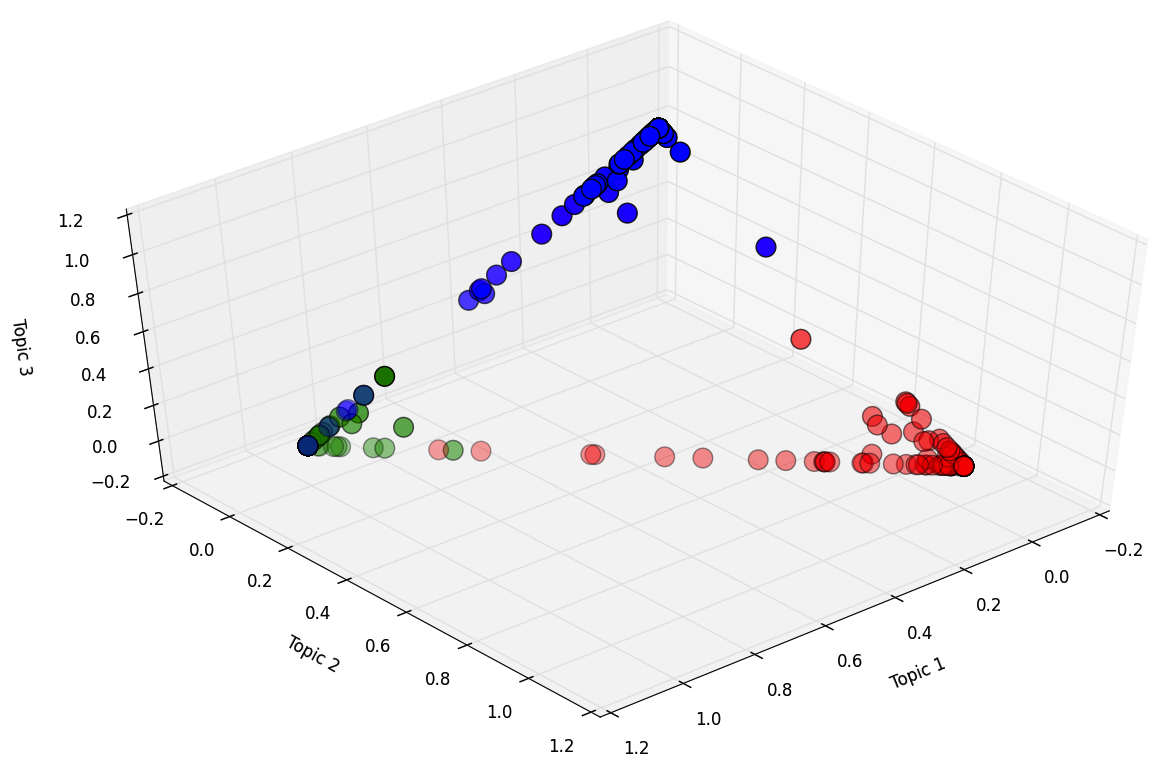
\includegraphics[width=\textwidth]{figs/classicalpha01beta02.png}
                \caption{$\alpha=0.1,\;\beta=0.2$}
                \label{fig:tiger}
        \end{subfigure}
        
        \begin{subfigure}[b]{0.5\textwidth}
                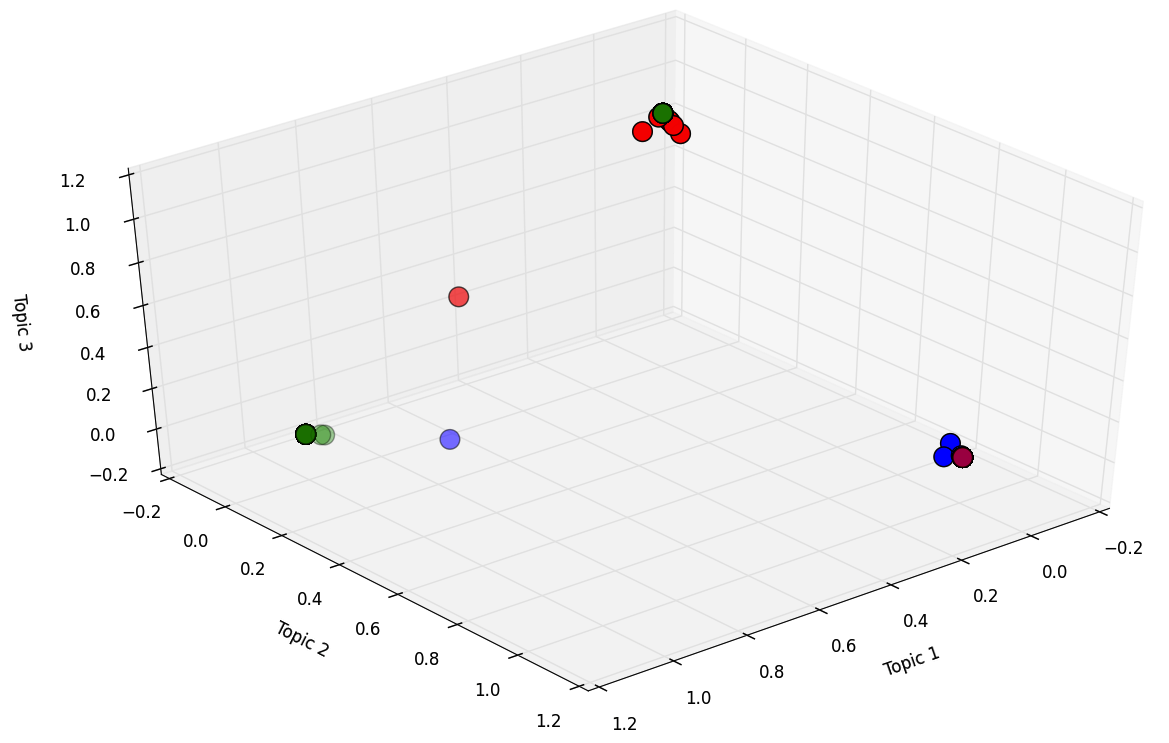
\includegraphics[width=\textwidth]{figs/classicalpha001beta2.png}
                \caption{$\alpha=0.01,\;\beta=2.$}
                \label{fig:mouse}
        \end{subfigure}%
        ~ %add desired spacing between images, e. g. ~, \quad, \qquad etc.
          %(or a blank line to force the subfigure onto a new line)
                  \begin{subfigure}[b]{0.5\textwidth}
                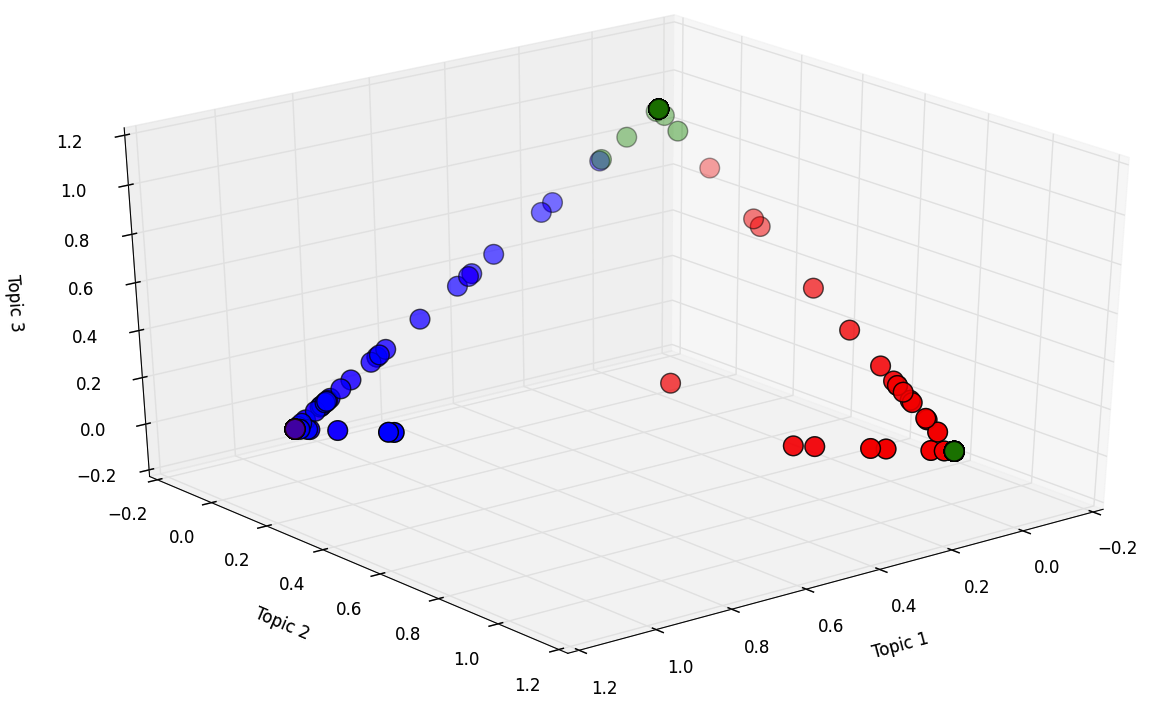
\includegraphics[width=\textwidth]{figs/classicalpha001beta02.png}
                \caption{$\alpha=0.01,\;\beta=0.2$}
                \label{fig:mouse}
        \end{subfigure}
        \caption{Distribution of documents after training on classic400 dataset. Each document is represented by its distribution over 3 topics.}
        \label{figClassicDist}
\end{figure}


\subsection{DailyKOS}
The number of documents and words in this dataset are given in table \ref{tableDatasetStats}. These are  documents mainly with political theme, however we also found rare occurrences of words such as \emph{sport}. Training on this document is a challenge of the large number of words and wide range of topics. The large number of words and topics results in slow training. Also the large number of topics makes discovery of rare topics hard for LDA. We train the model with different number of epochs ranging from 10 to 300 and number of topics ranging from 3 to 20. Table \ref{tableDKTopWords} shows the 
top words for a model trained with 20 topics and 300 epochs. These words make sense, for example topic 1 is about military , topic 2 is about crime and topic 3 is about weather.

We also try to plot the documents in 3D space, similar to figure \ref{figClassicDist}. However since the number of topics for this model is large, we have to reduce the dimensions for visualization. We used PCA and non-metric MDS for dimension reduction, however the documents in the plots were not well separated. That is because projection to lower dimension looses the sparseness of the documents.



\begin{table}[h!]
\begin{center}
\begin{tabular}{| c | p{12cm} |}
\hline
\textbf{Topic}& \textbf{Top 20 Words}  \\ \hline
\textbf{1}&bush, iraq, war, president, administration, kerry, bushs, people, time, draft, united, general, vote, media, years, americans, nation, states, military, nations\\ \hline
\textbf{2}& ban, assault, gun, weapons, law, canadians, laws, support, disagree, drug, fear, unsure, pass, groups, federal, expire, claims, crime, license, stated
\\
 \hline
\textbf{3}&summer, south, freedom, years, janklow, air, america, radio, time, june, numbers, fahrenheit, registered, white, mississippi, vance, fec, driving, april, meteor\\
 \hline

\textbf{4}&november, poll, senate, republicans, bush, electoral, polls, account, governor, house, democratic, voting, challengers, election, democrats, primary, kerry, voter, vote, economy
\\
 \hline

\textbf{5} &  bulb, cohen, reagan, energy, dkos, majette, weve,
 burt, hampshire, electricity, lightbulb, chandler,
 reynolds, impact, vision, important, kerr, space,
 real, endorsement
\\
 \hline

\textbf{6} &  brokaw, islam, islamic, democratic, sharpton,
 candidates, policy, posting, apparently, youre, nation,
 break, difference, exchange, philip, applause, morris,
 cbs, laughter, smoking
\\
 \hline
 
 
 
\end{tabular}
\caption{Top 20 words for 6 randomly selected topics in DailyKOS dataset. These topics make sense, for example topic 1 is military, topic 2 is crime and topic 3 is weather.}
\label{tableDKTopWords}
\end{center}
\end{table}


\section{Discussion}
In this paper, we described the details of training of an LDA model for document topic modeling. We saw that for an unsupervised learning problem such as topic discovery, LDA can be used to model the documents and its topics. We used Gibbs sampling to train a collapsed version of the model. For two datasets, we saw that our model can predict meaningful topics and discover an sparse representation of documents in topic space. For classic400 dataset, the model predicted the true topic for each document with more that 97\% accuracy.

One of the challenges when doing unsupervised training for model, is to determine the stopping criteria. This is the point in training where the model starts to over-fit the training data. We saw that Harmonic mean can't provide much information about the convergence because it converges very fast. In our experiments, we found that Gibbs sampling in the first few epochs do not provide any structure on the topic distribution in documents. Therefore, we let the Gibbs sampling run for 500 epochs.  

For DailyKOS dataset, we were dealing with a large number of words and topics. We discovered that training with small number of topics for this dataset results in mixed topics that are not separated. So we performed the training with large number of topics and the model discovered meaningful and well-separated topics. In order to get better results, we have to increase the number of epochs which leads to slower training. For this reason, we selected a random sub sample of documents in this dataset in order to perform training in reasonable time. Despite sampling, the model learned meaningful topics of words.


Because of the nature of problem, that deals with huge datasets, the algorithm is slow. In order to improve the speed, many algorithms have been proposed. In conventional Gibbs sampling methods (such as the one implemented here), training LDA require $O(K)$ per sample where $K$ is the number of topics. Reference \cite{fastlda} proposes a method which requires less than $K$ operations for each round of sampling. This method is based on the observation that the sampling distributions are frequently skewed such that most of the probability distribution is concentrated on a small fraction of the total number of topics $K$. This allows to order the sampling operations such that on average only a fraction of the $K$ topic probabilities need to be calculated.


\begin{thebibliography}{9}
\bibitem{fastlda}
Porteous, Ian, et al. "Fast collapsed gibbs sampling for latent dirichlet allocation." Proceedings of the 14th ACM SIGKDD international conference on Knowledge discovery and data mining. ACM, 2008.


\bibitem{harmonic}
Newton, Michael A., and Adrian E. Raftery. "Approximate Bayesian inference with the weighted likelihood bootstrap." Journal of the Royal Statistical Society. Series B (Methodological) (1994): 3-48.
APA	

\bibitem{wallach}
Wallach, Hanna M., et al. "Evaluation methods for topic models." Proceedings of the 26th Annual International Conference on Machine Learning. ACM, 2009.

\end{thebibliography}




\end{document}
